\documentclass[../../main.tex]{subfiles}
\begin{document}

\paragraph{【新課程】}
{\bf [解]}
接点の$x$座標を$t$ ($t>0$)とする．
$y = ax^2$について$y' = 2ax$，$y = \log_e x$について$y' = \dfrac{1}{x}$であるから，これら$2$つのグラフが点$(t, at^2)$で接するための必要十分条件は
\begin{align}
  \begin{cases}
    at^2 = \log_e t \\
    2at = \dfrac{1}{t}
  \end{cases}
  \iff
  at^2 = \log t = \dfrac{1}{2}
\end{align}
である．

二つ目の等号より
\begin{align}
  t = e^{1/2} \label{eq:1}
\end{align}
である．これを一つ目の等号に代入して
\begin{align}
  a = \dfrac{1}{2t^2} = \dfrac{1}{2e} \label{eq:2}
\end{align}
である．

さらに，この時のグラフは下図のようになる．
接点の座標は$\left(\sqrt{e}, \dfrac{1}{2}\right)$であり，$y=\log_e x$と$x$軸の交点は$(1, 0)$である．

\begin{figure}[htb]
  \centering
  \begin{tikzpicture}[scale=2.2, >=stealth, every node/.style={font=\small}]

    % --- 1. 定数の定義 ---
    % e = 2.7182818, sqrt(e) = 1.64872
    % a = 1 / (2e)
    \def\tVal{1.64872} % sqrt(e)
    \def\aVal{0.18394} % 1/(2*e)

    % --- 2. 面積 S の領域塗りつぶし ---
    % y = ax^2 (0 -> sqrt(e)) と y = ln(x) (1 -> sqrt(e))、および x 軸 (0 -> 1)
    \fill[pattern=north east lines, pattern color=blue!50]
    (0,0) -- plot[domain=0:\tVal, samples=60] (\x, {\aVal * \x * \x})
    -- plot[domain=\tVal:1, samples=60] (\x, {ln(\x)})
    -- cycle;

    % --- 3. 座標軸 ---
    \draw[->, thick] (-0.3, 0) -- (2.6, 0) node[right] {$x$};
    \draw[->, thick] (0, -0.9) -- (0, 1.2) node[above] {$y$};
    \node[below left] at (0, 0) {$O$};

    % --- 4. 関数の描画 ---
    % 放物線 y = a x^2
    \draw[very thick, blue!80!black, domain=0:2.3, samples=80]
    plot (\x, {\aVal * \x * \x}) node[above] {$y = ax^2$};

    % 対数目盛 y = log_e x
    \draw[very thick, red!80!black, domain=0.42:2.3, samples=80]
    plot (\x, {ln(\x)}) node[right] {$y = \log_e x$};

    % 共通接線 (傾き 1/sqrt(e), 接点 (sqrt(e), 1/2))
    % y - 1/2 = 1/sqrt(e) * (x - sqrt(e)) = x/sqrt(e) - 1/2
    \draw[thick, gray!60, dashed, domain=0.7:2.4]
    plot (\x, {\x / \tVal - 0.5});

    % --- 5. 補助点線と座標の投影 ---
    \draw[dashed, gray!80!black] (\tVal, 0) -- (\tVal, 0.5) -- (0, 0.5);

    % --- 6. 点のプロットとラベル ---
    % 接点
    \fill[purple!80!black] (\tVal, 0.5) circle (1.1pt);
    \node[above left=1pt, purple!80!black] at (\tVal, 0.5) {$\left(\sqrt{e},\,\frac{1}{2}\right)$};

    % 軸上の交点・目盛り
    \fill (1, 0) circle (1.0pt);
    \node[below=2pt] at (1, 0) {$1$};
    \node[below=2pt] at (\tVal, 0) {$\sqrt{e}$};
    \node[left=2pt] at (0, 0.5) {$\frac{1}{2}$};

    % 領域ラベル S
    \node[fill=white, inner sep=1.5pt, font=\normalsize\bfseries] at (1.05, 0.16) {$S$};

  \end{tikzpicture}
  \caption{$y=ax^2$ と $y=\log_e x$ の接点および囲まれる図形 $S$}
  \label{fig:parabola_log_area}
\end{figure}

この時，求める面積$S$は
\begin{align}
  S
  &= \int_0^{t} ax^2 \, dx - \int_1^{t} \log x \, dx \\
  &= \left[ \dfrac{a}{3}x^3 \right]_0^{t} - \Bigl[ x(\log_e x - 1) \Bigr]_1^{t} \\
  &= \dfrac{at^3}{3} - t\left(\log t - 1 \right) -1 \\
  &= \dfrac{1}{6e} \cdot e\sqrt{e} - \sqrt{e}\left(\dfrac{1}{2} - 1\right) - 1 \\
  &= \dfrac{\sqrt{e}}{6} + \dfrac{\sqrt{e}}{2} - 1  \\
  &= \dfrac{2}{3}\sqrt{e} - 1 \tag{答}
\end{align}
である．

\paragraph{【旧課程】}
$f(x) = 2\sin x$，$g(x) = a - \cos 2x$とおく．
導関数はそれぞれ
\begin{align}
  \begin{cases}
    f'(x) = 2\cos x \\
    g'(x) = 2\sin 2x = 4\sin x \cos x
  \end{cases} \label{eq:3}
\end{align}
である．
$0 \leqq x \leqq 2\pi$において，これら$2$つのグラフが点$(t, 2\sin t)$で接するための必要十分条件は
\begin{align}
  \begin{cases}
    2\sin t &= a - \cos 2t \\
    2\cos t &= 4\sin t \cos t
  \end{cases}
  \label{eq:4}
\end{align}
である．第$2$式より
\begin{align}
  2\cos t (1 - 2\sin t) = 0 \label{eq:5}
\end{align}
より，$\cos t = 0$ または $\sin t = \dfrac{1}{2}$ である．
$0 \leqq t \leqq 2\pi$の範囲で場合分けを行う．

\subparagraph{$1^\circ$ $\cos t = 0$のとき}

この時$t = \dfrac{\pi}{2}$または$t = \dfrac{3\pi}{2}$である．
\begin{itemize}
  \item $t = \dfrac{\pi}{2}$のとき: $\sin\dfrac{\pi}{2} = 1$，$\cos 2t = \cos\pi = -1$であるから，第$1$式より
    \begin{align}
      2(1) = a - (-1) \Longleftrightarrow a = 1
    \end{align}
    となり，接点は$\left(\dfrac{\pi}{2}, 2\right)$である．
  \item $t = \dfrac{3\pi}{2}$のとき: $\sin\dfrac{3\pi}{2} = -1$，$\cos 2t = \cos 3\pi = -1$であるから，第$1$式より
    \begin{align}
      2(-1) = a - (-1) \Longleftrightarrow a = -3
    \end{align}
    となり，接点は$\left(\dfrac{3\pi}{2}, -2\right)$である．
\end{itemize}

\subparagraph{$2^\circ$ $\sin t = \dfrac{1}{2}$のとき}
$t = \dfrac{\pi}{6}$または$t = \dfrac{5\pi}{6}$である．
このとき$\cos 2t = 1 - 2\sin^2 t = 1 - 2\left(\dfrac{1}{2}\right)^2 = \dfrac{1}{2}$であるから，第$1$式より
\begin{align}
  2 \cdot \dfrac{1}{2} = a - \dfrac{1}{2} \Longleftrightarrow a = \dfrac{3}{2}
\end{align}
となり，接点は$\left(\dfrac{\pi}{6}, 1\right)$および$\left(\dfrac{5\pi}{6}, 1\right)$の$2$点である．\casesend

以上より，求める$a$の値は
\begin{align}
  a = -3, \ 1, \ \dfrac{3}{2} \tag{答}
\end{align}
である．各場合の$0 \leqq x \leqq 2\pi$におけるグラフは以下の通りである．

\begin{figure}[h]
  \centering
  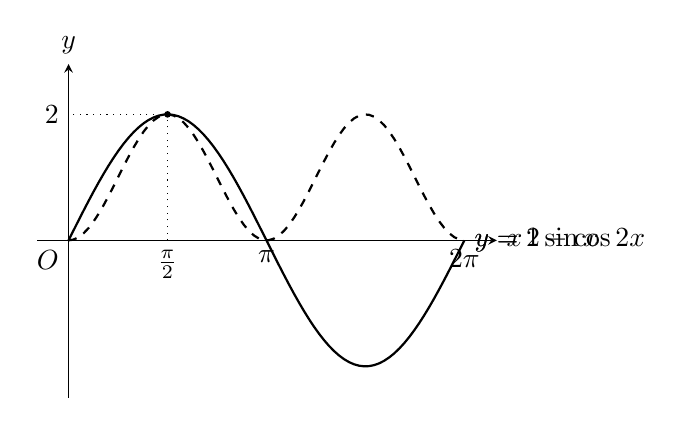
\begin{tikzpicture}[scale=0.8, >=stealth]
    \draw[->] (-0.5,0) -- (6.8,0) node[right] {$x$};
    \draw[->] (0,-2.5) -- (0,2.8) node[above] {$y$};
    \node[below left] at (0,0) {$O$};
    \draw[thick, domain=0:6.283, samples=80] plot (\x, {2*sin(\x r)}) node[right] {$y=2\sin x$};
    \draw[thick, dashed, domain=0:6.283, samples=80] plot (\x, {1 - cos(2*\x r)}) node[right] {$y=1-\cos 2x$};
    \draw[dotted] (1.571, 0) node[below] {$\frac{\pi}{2}$} -- (1.571, 2) -- (0, 2) node[left] {$2$};
    \fill (1.571, 2) circle (1.5pt);
    \node[below] at (3.142, 0) {$\pi$};
    \node[below] at (6.283, 0) {$2\pi$};
  \end{tikzpicture}
  \caption{$a=1$のときのグラフ（接点$\left(\dfrac{\pi}{2}, 2\right)$）}
\end{figure}

\begin{figure}[h]
  \centering
  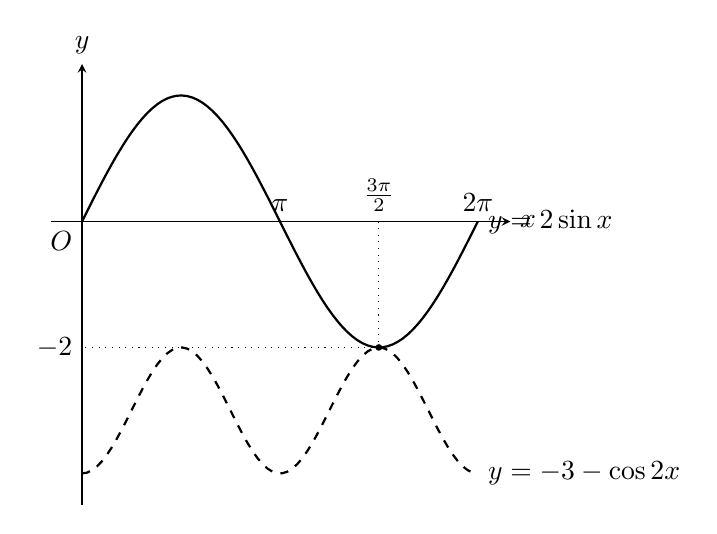
\begin{tikzpicture}[scale=0.8, >=stealth]
    \draw[->] (-0.5,0) -- (6.8,0) node[right] {$x$};
    \draw[->] (0,-4.5) -- (0,2.5) node[above] {$y$};
    \node[below left] at (0,0) {$O$};
    \draw[thick, domain=0:6.283, samples=80] plot (\x, {2*sin(\x r)}) node[right] {$y=2\sin x$};
    \draw[thick, dashed, domain=0:6.283, samples=80] plot (\x, {-3 - cos(2*\x r)}) node[right] {$y=-3-\cos 2x$};
    \draw[dotted] (4.712, 0) node[above] {$\frac{3\pi}{2}$} -- (4.712, -2) -- (0, -2) node[left] {$-2$};
    \fill (4.712, -2) circle (1.5pt);
    \node[above] at (3.142, 0) {$\pi$};
    \node[above] at (6.283, 0) {$2\pi$};
  \end{tikzpicture}
  \caption{$a=-3$のときのグラフ（接点$\left(\dfrac{3\pi}{2}, -2\right)$）}
\end{figure}

\begin{figure}[h]
  \centering
  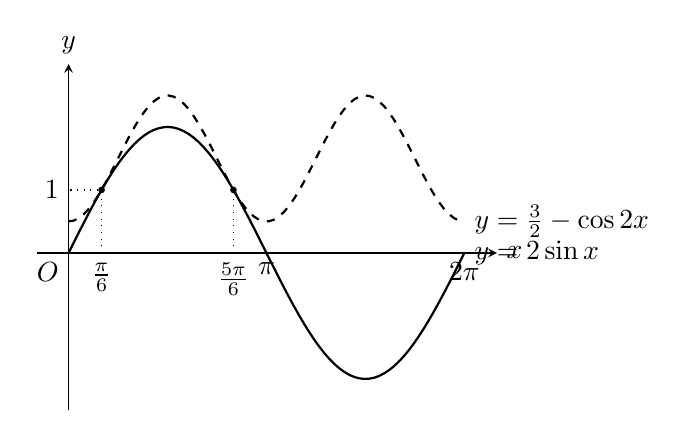
\begin{tikzpicture}[scale=0.8, >=stealth]
    \draw[->] (-0.5,0) -- (6.8,0) node[right] {$x$};
    \draw[->] (0,-2.5) -- (0,3.0) node[above] {$y$};
    \node[below left] at (0,0) {$O$};
    \draw[thick, domain=0:6.283, samples=80] plot (\x, {2*sin(\x r)}) node[right] {$y=2\sin x$};
    \draw[thick, dashed, domain=0:6.283, samples=80] plot (\x, {1.5 - cos(2*\x r)}) node[right] {$y=\frac{3}{2}-\cos 2x$};
    \draw[dotted] (0.524, 0) node[below] {$\frac{\pi}{6}$} -- (0.524, 1) -- (0, 1) node[left] {$1$};
    \draw[dotted] (2.618, 0) node[below] {$\frac{5\pi}{6}$} -- (2.618, 1);
    \fill (0.524, 1) circle (1.5pt);
    \fill (2.618, 1) circle (1.5pt);
    \node[below] at (3.142, 0) {$\pi$};
    \node[below] at (6.283, 0) {$2\pi$};
  \end{tikzpicture}
  \caption{$a=\dfrac{3}{2}$のときのグラフ（接点$\left(\dfrac{\pi}{6}, 1\right)$，$\left(\dfrac{5\pi}{6}, 1\right)$）}
\end{figure}

\end{document}
